% encoding: utf8
% !TEX encoding = utf8
% !TeX spellcheck = pl_PL

% STRONA TYTUŁOWA


\includepdf{pdf/strona_tytulowa.pdf}
\clearpage\mbox{}\thispagestyle{empty}\newpage


% AUTOR


%\par
%\vspace{0.2\baselineskip}
%\hfill\parbox{15em}{{\small\dotfill}\\[-.3ex]
%	\centerline{\footnotesize podpis studenta}}\par
%
%\vspace{1\baselineskip}

\clearpage\mbox{}\newpage


% STRESZCZENIE POLSKIE

\vspace*{\baselineskip}
\begin{center}
	{\large\bfseries Streszczenie}\par\bigskip
\end{center}
\noindent{\bf Tytuł}: {\itshape Chwytanie przedmiotów w~robocie sterowanym impedancyjnie}
\\\\
{
	Zastosowanie siłowych praw sterowania daje możliwość łatwej kooperacji robota z~człowiekiem. Jednym z~nich jest sterowania impedancyjne. W~trakcie manipulacji z~chwytaniem przedmiotów okazuje się, że siła grawitacji przedmiotu nie jest kompensowana przez silniki robota. Celem pracy jest implementacja algorytmu kompensującego wpływ siły grawitacji chwytanego przedmiotu o~nieznanych parametrach masy i~inercji w~robocie sterowanym impedancyjnie.
	
	Wykorzystywany do badań robot Velma zbudowany jest z~dwóch ramion LWR-4 osadzonych na ruchomym korpusie. Oprogramowanie robota zostało zaprojektowane przy pomocy teorii agenta upostaciowionego i~zaimplementowane przy użyciu struktury ramowej FABRIC. Robot korzysta z~impedancyjnego prawa sterowania i~samodzielnie kompensuje siłę grawitacji ramion. 
}\\\\
\vspace*{0.6\baselineskip}
\noindent{\bf Słowa kluczowe}: {\itshape Velma, FABRIC, ROS, LWR}

\clearpage\mbox{}\newpage


% STRESZCZENIE ANGIELSKIE
\vspace*{\baselineskip}
\begin{center}
	{\large\bfseries Abstract}\par\bigskip
\end{center}
\noindent{\bf Title}: {\itshape Grasping objects in impedance control robot}
\\\\
{ 
	The use of impedance and force control gives the possibility of easy cooperation between a robot and a human being. During manipulation with gripping objects, it appears that the gravitational force of the object is not compensated by the robot motors. The aim of this thesis is to implement an gravity compensation algorith for impdance control with unknown tool parameters.
	
	The Velma robot used for research. It consists of two LWR-4 arms mounted on a movable body. The robot software has been designed with embodied agent theory and implemented using the FABRIC framework. The robot uses impedance control and independently compensates gravity of the arms.
}\par
\vspace*{1\baselineskip}
\noindent{\bf Keywords}: {\itshape Velma, FABRIC, ROS, LWR}

\clearpage\mbox{}\newpage


% OSWIADCZENIE
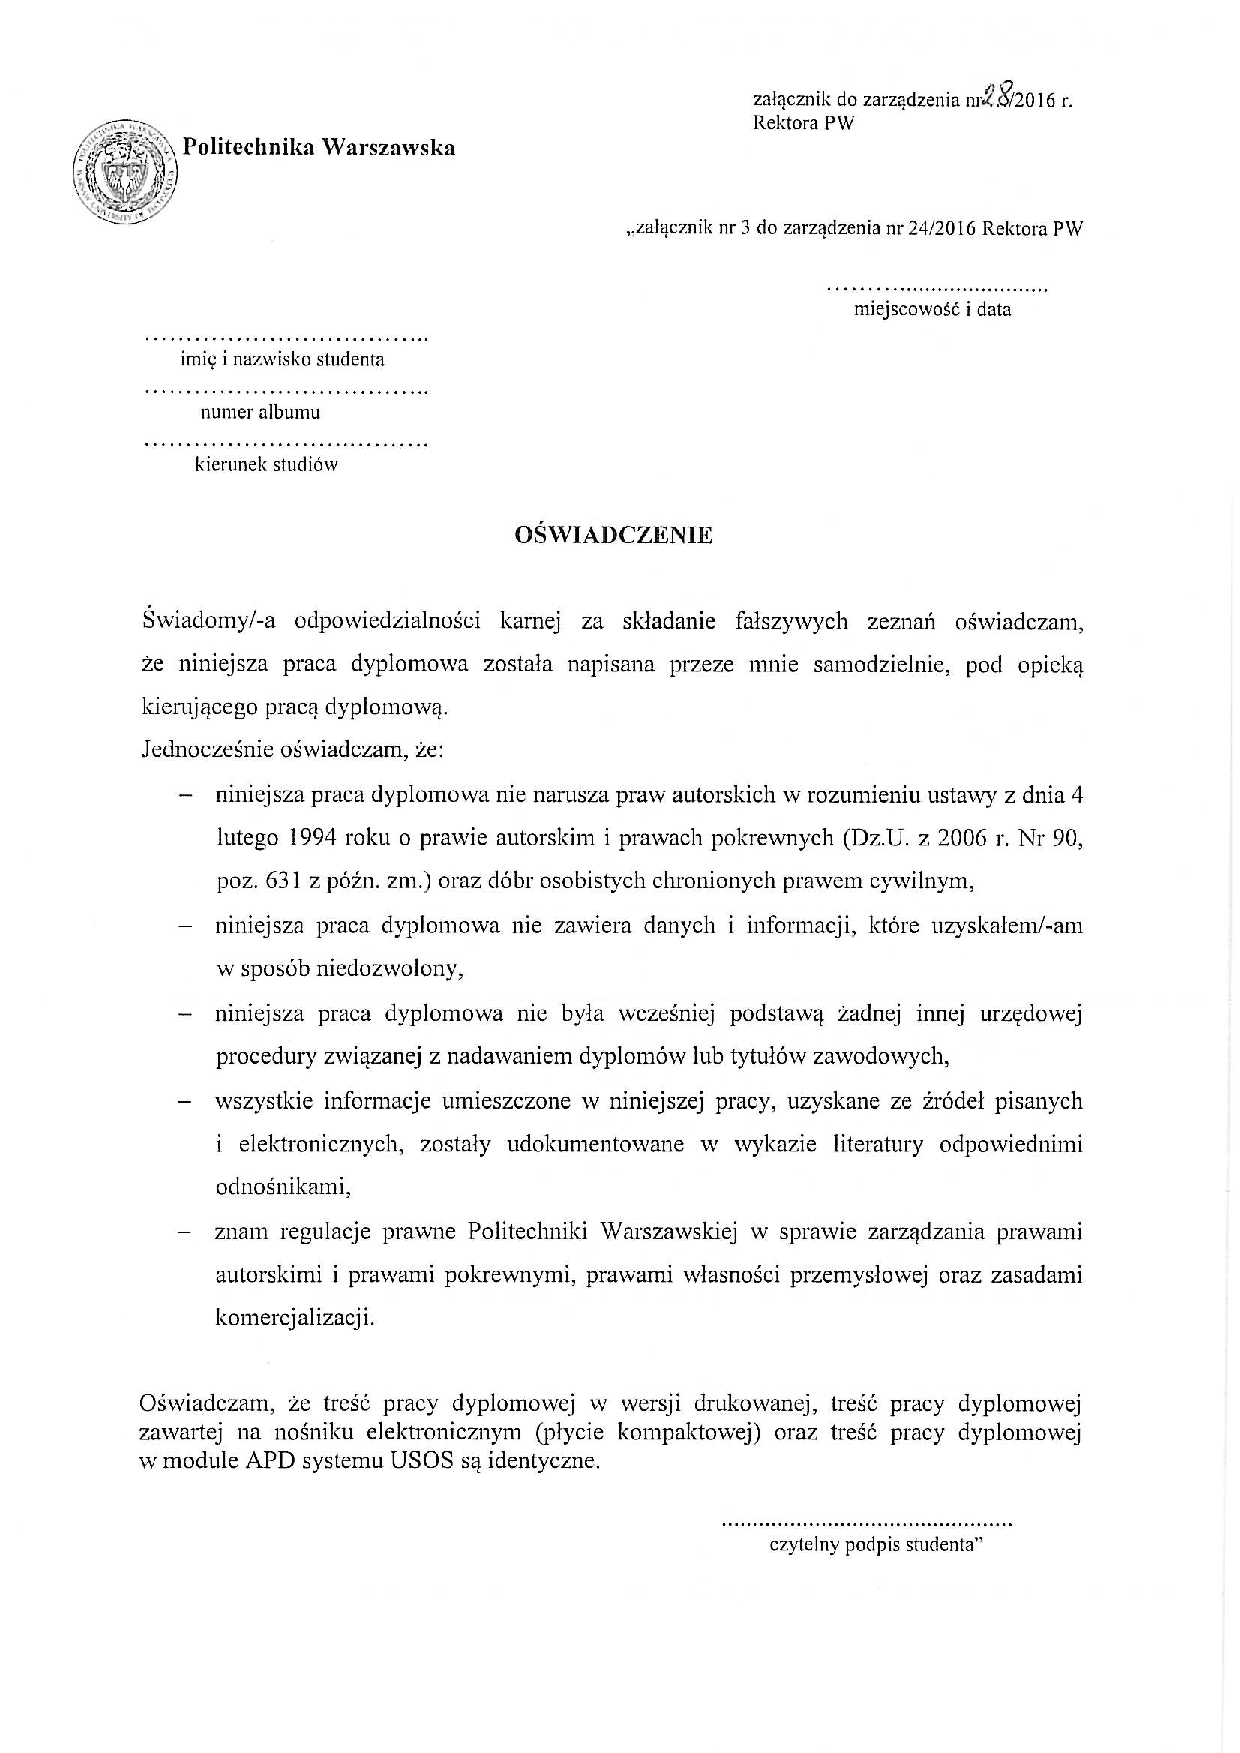
\includepdf[pagecommand={}]{pdf/oswiadczenie.pdf}
\clearpage\mbox{}\newpage


% PODZIĘKOWANIA


